\section{The Proposed Belovezha Architecture}\label{sec:chap05:proposed_work}
\begin{figure}[h]
    \centering
    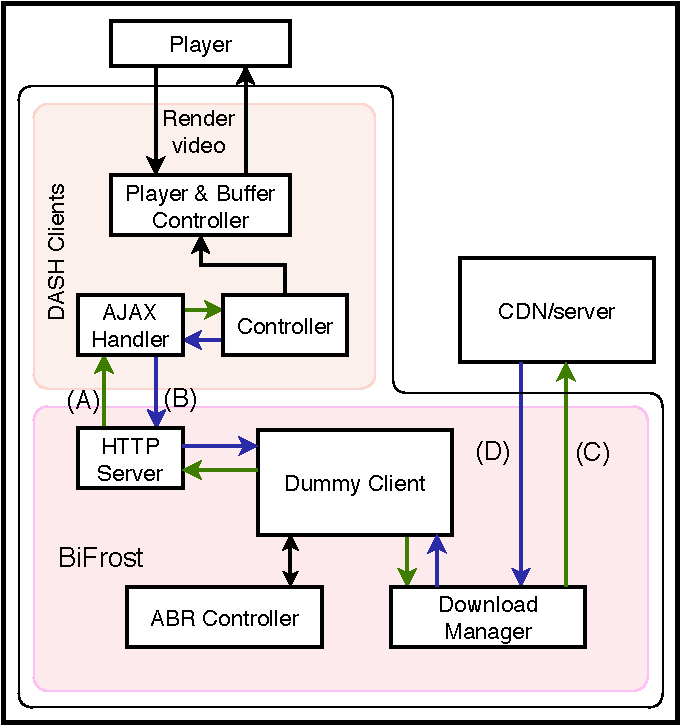
\includegraphics[width=\linewidth]{./images/playerDiagram_split.pdf}
    \caption{Proposed \bel\ architecture - a Split DASH model. There is a Dumb DASH Client at the user end and a Smart DASH Intelligent Proxy Server, \servname\, between the CDN server and the client.}
    \label{fig:chap05:splitDASH}
\end{figure}
In this section, we explain the architecture of \bel, which comes with the following major modifications in the DASH architecture:
\begin{enumerate}[(i)]
    \item the smart \ac{DASH} client is replaced with a dumb client in \bel , and
    \item an intelligent DASH proxy server, named \servname\, is introduced between the \ac{CDN} server and the client.
\end{enumerate}\
The resulting \bel\ architecture is shown in Fig.~\ref{fig:chap05:splitDASH}. The dumb client does not take any decisions related to the choice of the chunk bitrates. It simply controls the video playback while depending on \servname, to fetch the chunks from the CDN server. To assist \servname\ in taking bitrate decisions for future video chunks and delivering the same, the client reports - (a) its current playback buffer status, \am{(b) current playback time, (c) total stall time} and (d) its previous download history, to \servname\ every time it sends a request to \servname\ for video-segment download. \\
\indent \textcolor{red}{AM: Every time \servname\ receives a request from the client, it combines the information sent by the client into a `\textit{server state}'}. \textcolor{blue}{ It uses this server state to decide the audio and the video quality of the next video chunk to be downloaded. It has been discussed earlier that \servname\ will be co-located either with a  \ac{CDN} server or a \ac{BS}. However, during the course of travel, a mobile user does not connect to the same \ac{CDN} server or \ac{BS}. Evidently, it will not always connect to the same \servname\ server, for which the latter has been designed to be stateless.  So, \servname\ forwards the previous download history (received earlier from the client) to the client along with the current video segment. In addition, it also sends the time the client must wait before sending the next request for segment download.\\
\indent The next two sections provide a detailed description of the design and functioning of both the \bel\ client and the server.}
\subsection{The Belovezha Client}
The \bel\ client has three fundamental modules - a) a playback and buffer controller, b) a client controller and c) an AJAX manager.
\subsubsection{Playback and Buffer Controller}
    The \textit{playback and buffer controller} controls the video playback at the native player using the Source Buffer APIs of HTML5 Media Source Extension. It acts as an interface between the native player and the client controller.
\subsubsection{Client Controller}
The \textit{Client controller} supervises the functioning of the entire client. It starts the moment the client starts up and  initiates communication with the \bel\ server - \servname. It prepares all the requests to be sent to \servname, parses the received responses, and then  follows the instructions received. When the response contains any media segment, it feeds the media segment to the buffer controller. The client controller also maintains a record of the playback buffer status, and the current segment download information over link between the client and \servname.
\subsubsection{AJAX Controller}
The \textit{AJAX controller} handles the communication between \servname\ and the client. It monitors the communication continuously and records all the events. If a communication stays unresponsive for a threshold time, it aborts the communication and starts it again. The AJAX controller aborts communication by itself instead of relying on the native connection timeout mechanism to have more control, which makes the client robust and tolerant to network failures.
\subsection{The Belovezha server - BiFrost}
\begin{figure*}[h]
    \centering
    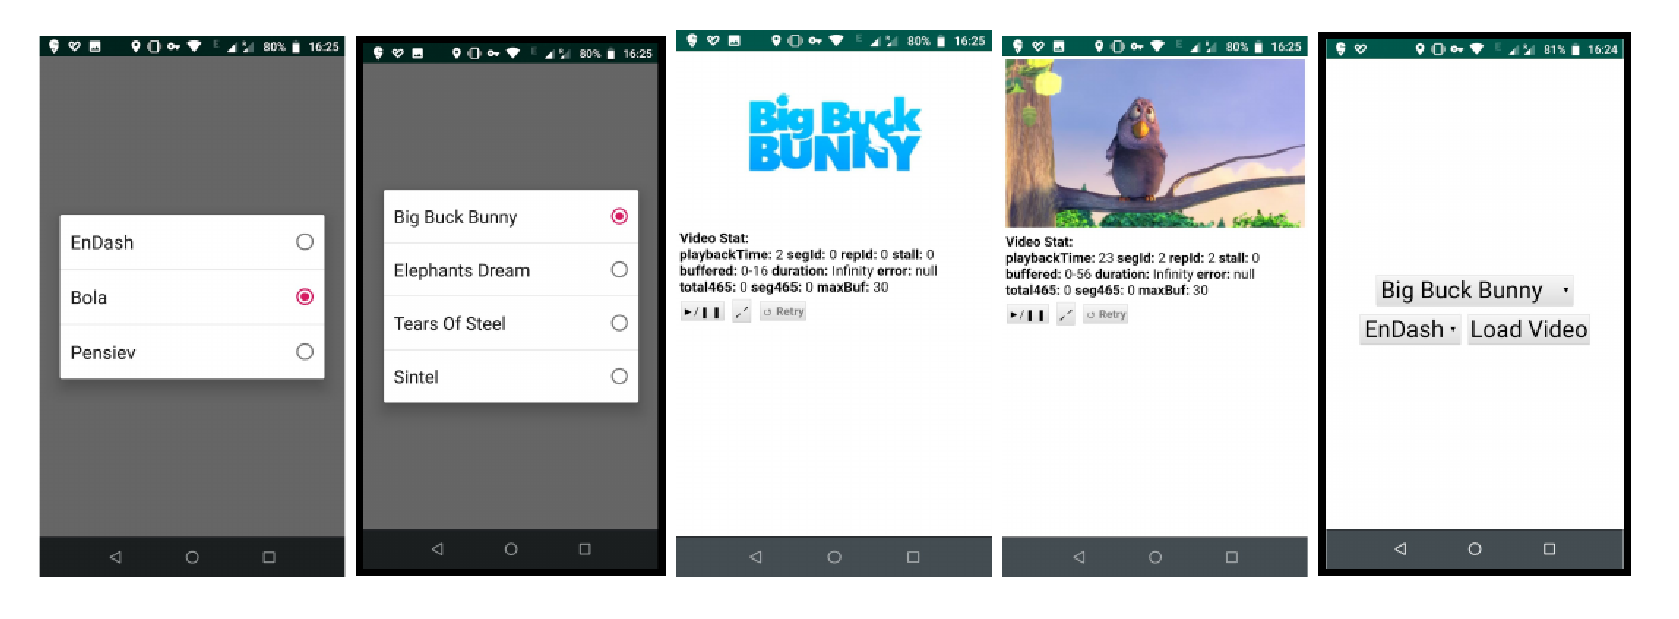
\includegraphics[width=0.8\textwidth]{images/App_Specs.eps}
    \caption{A snapshot of the \bel\ Player}
    \label{fig:chap05:bel_client}
\end{figure*}
 The heart of \bel\ is its middleware-server - \servname, which is an intelligent \ac{DASH} proxy server, It is essentially an HTTP server, albeit with a few extra capabilities. The major modules in \servname are -  a) an HTTP server,  b) a dummy client instance, and  c) the \ac{ABR} controller which houses the ABR algorithms.
\subsubsection{HTTP server}
The \textbf{HTTP server} module forms the front end of \servname. It maintains the TCP link with the client. For ease of implementation, everytime a new request arrives, \servname\ creates a new process in the HTTP-server. This allows the utilization of the multiple cores available in the system and serve multiple requests concurrently \am{AM:(we have to mention that we have developed server using python)}.

\subsubsection{Dummy Client}
To process the information received from the client, \servname\  creates a new instance of the client  at its end for every new service request. We refer to this instance as the dummy client. When \servname\ receives the request for the $n^{th}$ video segment download, there are two sets of information from the client - (a)  the current playback buffer status, and (b) the download information till the $(n-1)^{th}$ segment download (this can include the history for past $k$ segments. So, it generates a new server state including the aforementioned information. This is then forwarded to the \ac{ABR} controller for selecting the audio-video quality and the next sleep time duration of the client. When the bitrate decisions arrive from the \ac{ABR} controller, the dummy client instance uses the download manager to download the segment from the \ac{CDN} server. It then prepares the HTTP response, which includes (a) the downloaded segment, (b) the previous download history received from the client, and (c) the sleep time duration.
\subsubsection{ABR Controller}  The ABR controller is a collection of pluggable ABR algorithms. The dummy controller feeds the server state containing the playback and download information to the ABR controller. These metrics are used by the \ac{ABR} algorithm placed inside the ABR controller to take the bitrate decisions. There may be different types of ABR algorithms - (i)rate based, (ii) buffer based, (iii) hybrid, i.e., both rate and buffer based, (iv) quality based, (v) learning based, etc. Some of these algorithms like~\cite{mao2017neural,Akhtar2018,Sengupta2018} needs the previous server state, in other words the download information, to calculate the output quality for the next segment.
\subsubsection{Download Manager}
Another module in the server is the \textbf{download manager} which downloads the segments from the CDN server. It also maintains a very basic LRU based caching to avoid downloading segments which have been already downloaded.
\subsection{Implementation}
The popularity of DASH, as discussed earlier, is primarily stimulated by the use of existing \ac{CDN} network and the interoperability of \ac{DASH}. In \bel\ the \ac{CDN} remains unchanged as before. In this section, we shall explain the implementation of the major modifications introduced by \bel, i.e., the \bel\ client and its \servname\ server.

% \am{Unlike DASH, the \bel\ has three primary components 1) CDN, 2) \servname\ proxy server and 3) a \cliname. Among these three components, the CDN is exactly same as normal DASH based services. It contains the streaming data and serve to the players. The \servname\ and the \cliname\ is the splitted version of smart DASH client. Here the \cliname\ is responsible for playing the video at the end user side, however, all the decision regarding quality selection and buffer managements are taken by the \servname. In this subsection we are going to discuss the implementation detail of the \cliname\ and \servname\ and the communication protocol between these the components.}

%\basabdatta{Need to know details from abhijit}

%\basabdatta{Need to know details from abhijit}
%\newcommand{\cliname}{dumb client}

\subsubsection{The \bel\ Client}
The \bel\ client has been developed as an HTML5 and Javascript based Android application. A snapshot of the client application is shown in Fig.2. Inside this application, the \textit{playback and buffer controller} at the client is an HTML5 video player with all playing options, such as play pause, and seek. Additionally, the video player also needs a video source, which can either be an HTTP video source or a source buffer. In this work, we use the Source buffer APIs since it offers a set of options  such as playing a video with partial data, changing video quality on the fly, etc. The  AJAX handler and the \textit{Client Controller}, which as mentioned earlier maintain the communication with \servname\  and follows and executes the instructions coming from the \servname, respectively, are both implemented using Javascript.
\subsubsection{The \bel\ Server - \servname}
The \servname\ server has been implemented to be hosted in an Amazon Web Server. Thr front end of \servname\ is an HTTP server module which maintains the communication with the client.  It has been implemented by extending the Python BaseHTTPServer module. As Python does not support true multi-threading, a new process is created with every new request that \servname\ receives. This allows the utilization of the multiple cores available in the system and serve multiple requests concurrently. Moreover, \servname\ maintains a unique dummy client and \ac{ABR} controller for each client. This allows \servname\ to serve multiple clients at a time. When the client is on the move both the dummy client and the \ac{ABR} controller has to migrate the current \servname\ server to the new \servname, while preserving their current state.\\
\indent For implementing the ML-assisted \ac{ABR} algorithms Tensorflow is used. In this work, we have implemented only Pensieve. \basabdatta{more to write}.
\subsection{Message Flow}
\indent To render clarity to the operation of \bel\ we have shown in Fig. \ref{fig:chap05:info_xchang} the information exchanges between the \bel\ client and \servname\ in detail. Before engaging in the flow of information between the \bel\ client and the \servname\ server, we introduce a few terms - \textbf{(a) Session}: A session is the time duration from the start to the end of a single video streaming. If the player is reloaded then a new session starts. \textbf{(b) State}: A state is a set of carefully chosen parameters of an ongoing process. The criteria for the choice of parameters is to ensure that the restart point of a process should be the previous instance and not the beginning. An example of a state is the serialized object of a class. On deserialization a user will be left with an exact copy of the previous object even if the process becomes different \basabdatta{ask abhijit}. \bel\ records the states of three different modules - (a) the \bel\ client (\basabdatta{specifics}), (b) the dummy client at \servname, and (c) the ABR controller at \servname.\textbf{(c)  Download Information}: The download information is recorded at the AJAX handler and includes the payload and the header size of both the client request and the \servname\ response. It also includes three timestamps, such as, (i) request sent (\basabdatta{ask abhiit}) (ii) first byte of the response received and (iii) the last byte of the response received. The size of each download information is approximately 40 Bytes.\\
\begin{figure}[h]
    \centering
    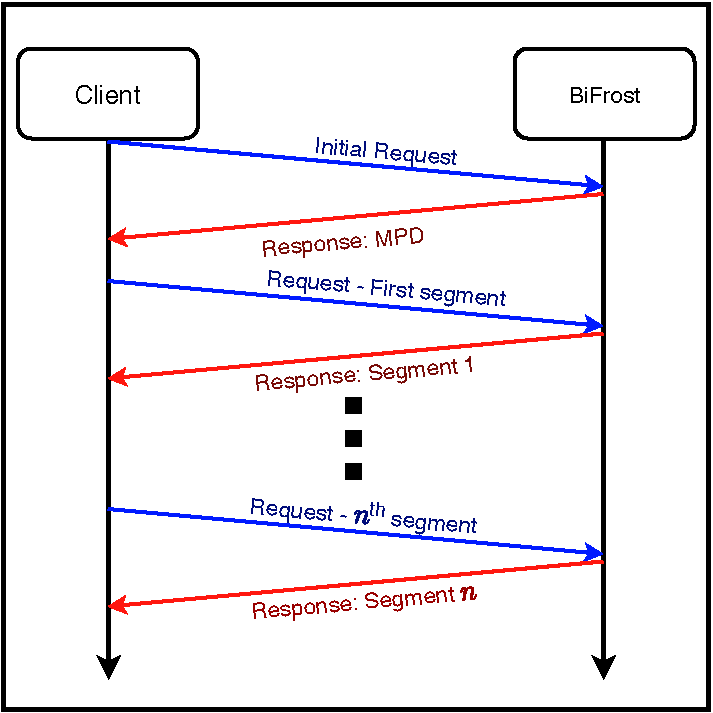
\includegraphics[width = 0.8\linewidth]{./images/splitDASHTransaction.pdf}
    \caption{The message flow between the client and the moderator server \servname\ of the \bel\ \acs{DASH} architecture. The demonstrated flow corresponds to a stateless \servname\ server. \servname\ can also be stateful.}
    \label{fig:chap05:info_xchang}
\end{figure}{}
\subsubsection{The Control Flow}
To \textit{initiate} a video streaming session the \bel\ client first places the request for the Media Presentation Description (MPD) of the target video to \servname. The MPD contains all information associated with the properties of the target video. At this stage, the playback buffer length is zero, and the \bel\ client has no download information or any information related to the video. When \servname\ receives the MPD request it creates (a) a dummy client object and (b) an \ac{ABR} object. For a non-MPD request both of these objects are either initiated with zeros or are empty. These are then piggybacked with the un-modified MPD as a blob and sent to the client.\\
\begin{figure}[h]
    \centering
    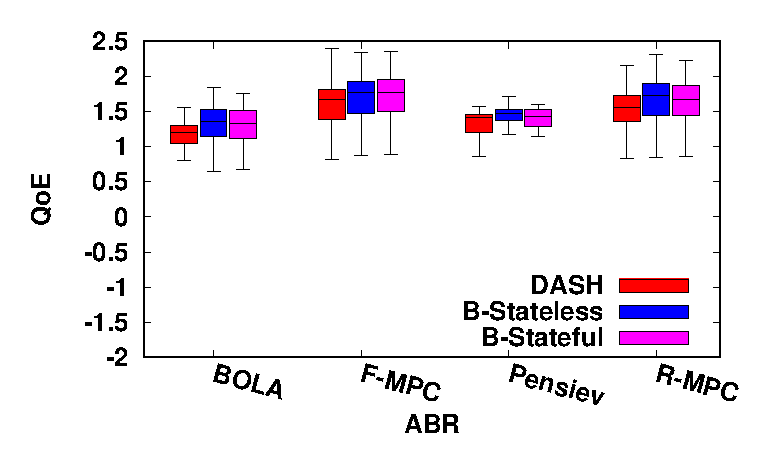
\includegraphics[width=0.5\textwidth]{images/qoeBox.eps}
    \caption{Box plot representing \acs{QoE} of users over different network conditions. The performance of both stateless and stateful \servname\ servers are captured.}
    \label{fig:chap05:result_qoe}
\end{figure}
\begin{figure}[h]
	\captionsetup[subfigure]{width=0.7\linewidth}
	\begin{center}
		\subfloat[\label{fig:chap05:result_bitrate}Average Bitrate]{
			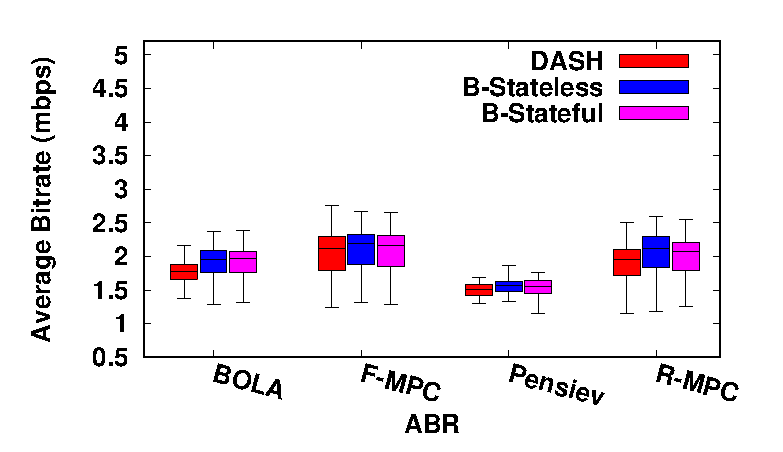
\includegraphics[width=0.49\linewidth]{images/avgQlBox.eps}
		}
%		\vspace{+5mm}
		\subfloat[\label{fig:chap05:result_smoothness}Average bitrate variation]{
			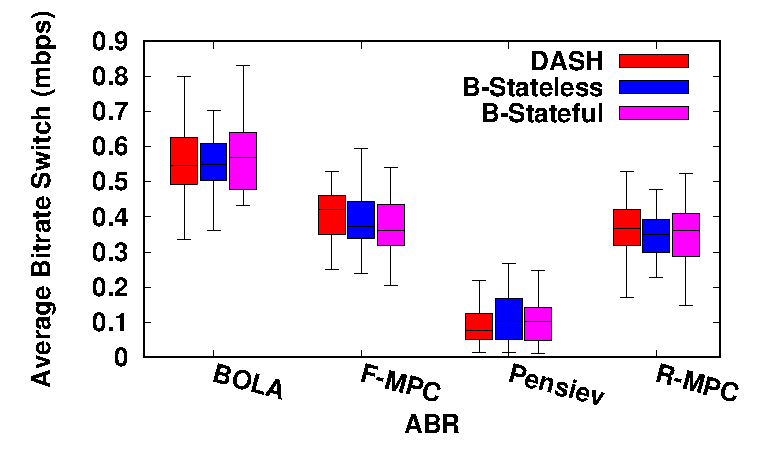
\includegraphics[width=0.49\linewidth]{images/avgQlVarBox.eps}
		}\\
%		\vspace{+5mm}
		\subfloat[\label{fig:chap05:result_stall}Average Rebufferring Time]{
			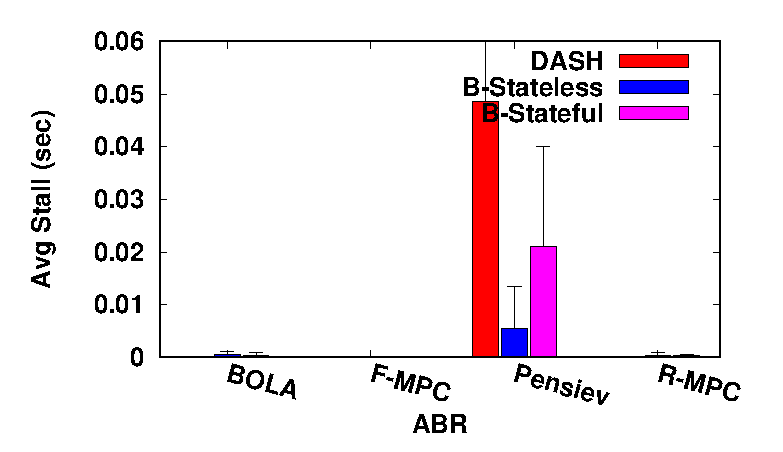
\includegraphics[width=0.3\linewidth]{images/avgStallsBox.eps}
		}
	\end{center}
	\caption{Individual QoE components}
\end{figure}
%\begin{figure*}[t]%
%\centering
%\subfigure[Average Bitrate]{%
% \label{fig:result_bitrate}%
%  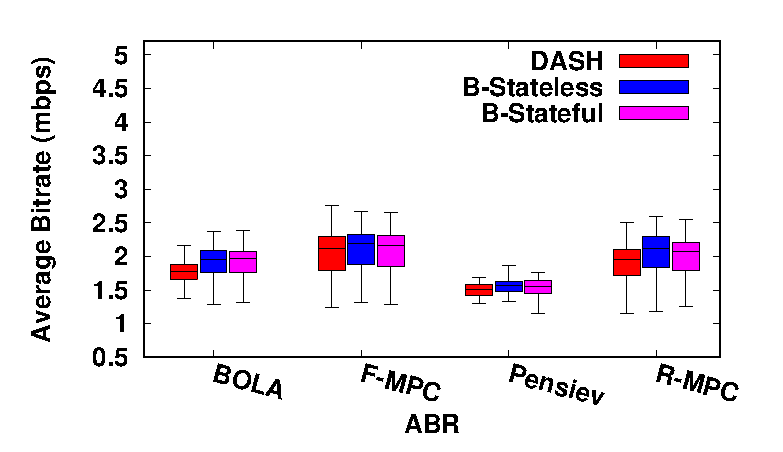
\includegraphics[width=0.3\textwidth]{images/avgQlBox.eps}}
%\hspace{0.1cm}
%\subfigure[Average bitrate variation]{%
% \label{fig:result_smoothness}%
% 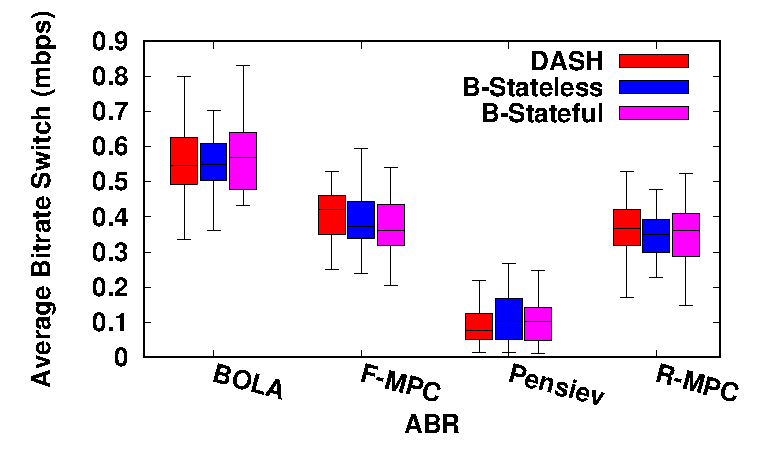
\includegraphics[width=0.3\textwidth]{images/avgQlVarBox.eps}
%}%
%\hspace{0.1cm}
%\subfigure[Average Rebufferring Time]{%
%\label{fig:result_stall}%
%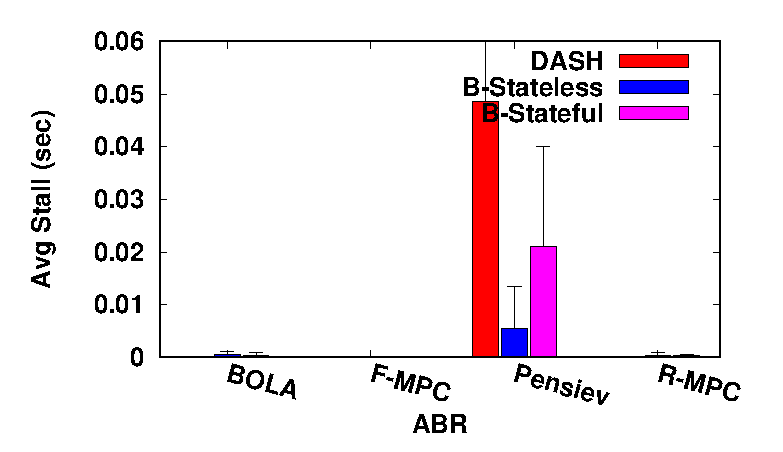
\includegraphics[width=0.3\textwidth]{images/avgStallsBox.eps}
%}
%\caption{Individual QoE components}\vspace*{-0.5cm}
%\end{figure*}
\indent Upon receiving the MPD, the client controller records the current download information associated with the MPD, and immediately forwards the request for the first video segment download. The auxiliary information sent by the client along with the request include the playback buffer length, the playback time, the current rebuffering time  and only one download information corresponding to the MPD.  For the first request, playback buffer length, playback time, and current rebuffering time are all equal to zero. In addition it also sends the blob (containing the previous instance of the dummy client and the ABR controller at \servname) along with the request. For a non-MPD request, the dummy client state is composed of the next segment number, the download quality of the last five segments, and the last five download information. The \ac{ABR} controller state is, however, dictated by the \ac{ABR} algorithm. For example, buffer based \ac{ABR} algorithms like BOLA \cite{Spiteri2016} does not need any prior information. However, algorithms like MPC \cite{yin2015control} and Pensieve \cite{mao2017neural} require a large set of input parameters for operation \\

\indent Once the request arrives at \servname, it first looks for the blob and responds with an error if the blob is absent. Otherwise it restores the dummy client object and the ABR controller object to their previous state using the information available in the blob. Only after restoring the previous instance, it then updates both of these two objects using the new set of information received from the client. The dummy controller then directs the \ac{ABR} controller, which replies with the audio and video quality of the next video segment.  The dummy controller also calculates the time that the \bel\ client should wait before sending the next request. We refer to this as the \textit{sleep time}, which is calculated as follows:\basabdatta{write equation} Once \servname\ arrives at these decisions, it fetches the video segment from the \ac{CDN} server at the quality prescribed by the \ac{ABR} controller. It then forwards the segment along with the dummy controller and ABR controller state as well as the sleep time to the client.\\
% \indent When the client receives the segment response, it forwards it to the player. Simultaneously it updates its own sleep time. An inherent assumption is that the \bel\ client sleeps during the entire download. When the last segment is downloaded \servname\ notifies the client by sending an {\tt End of Video (EoV)} flag the client. The session terminates either if the user chooses to end the session or if the video playing is over. In the latter case, it is terminated by the client. At this stage, the playback buffer length is zero. Thus, the auxiliary information sent by the client along with first segment download request includes the playback buffer status and the MPD download information. Using both of these, the dummy client instance at \servname\ creates a server state and forwards the same to the \ac{ABR} controller. Once the \ac{ABR} controller decides the audio-video quality for the next segment download, the dummy client instance (i) downloads the segment at the corresponding quality from the \ac{CDN} server, (ii) calculates the sleep time duration, (iii) forwards the segment to the client such that the previous download history (received from the client) and the sleep time duration is piggybacked with it. For downloading the $n^{th}$ segment, the client sends the history associated with the download of $(n-1)$ segments. The client may also send the history for $(n-1-k)$ to $(n-1)$ segments for $k = {0,1,\cdots,(n-k-2}$, albeit with some minor savings in the control channel overhead.\\
% \indent The sleep time duration depends on the buffer status and the current download. It is calculated as follows:
% % \begin{enumerate}[(i)]
% %     \item
% %     \item Upon receiving the MPD request, \servname\ prepares a new server state. It populates the state with the current download history and then  responds with an un-modified MPD for the video. If \servname\ is \textbf{stateless}, it pushes the server state to the client along with the MPD. Otherwise, if \servname\ is \textbf{stateful} then it stores the server state itself. Additionally, \servname\ also appends an identifier \textbf{X-Server-Type: Smart}, which indicates that the MPD is received from \servname\ and not the simple CDN server. This is the first instance where a bottleneck associated with the introduction of \servname\ as a middlebox is bypassed.
% %     \item Upon reception of the MPD, the client prepares the video element in \texttt{HTML} and requests \servname\ for the first video segment. Unlike in the conventional DASH protocol, the client does not specify the video/audio quality for the segment requested.
% %     \item When \servname\ is \textbf{stateless}, the client pushes the previous server state, containing the previous download history, along with the download request to \servname.
% %     \begin{itemize}
% %         \item Upon reception of the request, \servname\ looks for any old state in the request.
% %         \item If any such state is present, it expands it; otherwise, it creates a new state.
% %         \item  In a new server state, \servname\ includes the playback information and the download history received from the client along with the request. \servname\ then feeds these information to its \ac{ABR} algorithm to calculates the best quality for both audio and video segments.
% %     \end{itemize}

% %     \item In case where \servname\ is \textbf{stateful}, it stores its own previous states. So, when a new download request containing the current playback information arrives from the client, \servname\ uses the playback information and the download history in its stored server state to calculate the audio and video quality of the chunks to be fetched using an ABR algorithm.
% %     \item Once the quality is decided, \servname\ downloads the video segments at the calculated quality from the CDN/streaming (if not available in its cache) and forwards it to the client for reordering at the player. It also calculates the time for which the client should wait (i.e., the sleep time) before sending the next request to the moderator-server. It piggybacks the sleep time with the video chunks. \servname\ also adds the server state in case it has a stateless design.\basabdatta{BP: need to develop sleep time derivation formula.}
% % \end{enumerate}{}
% %   Most of the deterministic ABR algorithms do not require to maintain any state. Hence, \servname\ by default can be designed to be stateless. However, \ac{ABR} algorithms, such as Pensieve \cite{mao2017neural}, Oboe \cite{Akhtar2018} and HotDASH \cite{Sengupta2018}, need the information on past chunk downloads to decide the bitrate of future chunks. This gives rise to the need for recording the server state of \servname. If \servname\ is stateful, amount of control information exchanged is significantly reduced. If, on the other hand, \servname\ is stateless then its storage requirement reduces, however, at the cost of increased control information exchanges. \\
%   \indent We next describe implementation aspects of the \bel\ client and the server, i.e., \servname.

% % . We have this migration in the later part of this section.
% % server. Th recording the download information associated with every video segment download, etc.
% % \begin{enumerate}
% % 	\item {\bf Video playback handler:} It handles the . HTML5 provides a video player and several ways to control it. The controls are like, . The video player also need a video source. The HTML5 have several options for video source like http video source, source buffer. Among these video sources, the source buffer API is particularly interesting. It allows video player to play video with partial data, change the video quality and other feature on the fly. We utilize this API to change the quality whenever require. The video playback handler module handles all these tasks.
% % 	\item {\bf AJAX handler:} The segment download manager is implemented using AJAX api available in the JavaScript. This particular module handle communication between the \cliname and the \servname and keep log in form of download inform.
% % 	\item {\bf Controller:} All though the \cliname\ is dumb, it need a controller to follow and execute instruction from the \servname. The controller module exists to perform the task. It connect the video playback handler and the the AJAX handler. It create the request to send to the \servname\ and parse the response received from the \servname.
% % \end{enumerate}

% % \am{
% % We implement the \cliname\ using HTML5 and JavaScript. We have three basic module in our \cliname\ implementation:
% % \begin{enumerate}
% % 	\item {\bf Video playback handler:} It handles the HTML5 video player. HTML5 provides a video player and several ways to control it. The controls are like, play pause, seek. The video player also need a video source. The HTML5 have several options for video source like http video source, source buffer. Among these video sources, the source buffer API is particularly interesting. It allows video player to play video with partial data, change the video quality and other feature on the fly. We utilize this API to change the quality whenever require. The video playback handler module handles all these tasks.
% % 	\item {\bf AJAX handler:} The segment download manager is implemented using AJAX api available in the JavaScript. This particular module handle communication between the \cliname and the \servname and keep log in form of download inform.
% % 	\item {\bf Controller:} All though the \cliname\ is dumb, it need a controller to follow and execute instruction from the \servname. The controller module exists to perform the task. It connect the video playback handler and the the AJAX handler. It create the request to send to the \servname\ and parse the response received from the \servname.
% % \end{enumerate}
% % }
% % HTML5 provides Media Source Extension (MSE) to render multi-media in the browser. It also provides an API called Source Buffer API to control the playback buffers on the fly using JavaScript. This API allows users to add segmented video chunks on the fly or to change the audio video qualities. Most of the popular browsers (including webviews) in almost all the platforms support these APIs. So, in order to make \bel\ platform independent, we have implemented the \bel\ client using HTML5 and JavaScript.\\
% %\indent In our implementation, a native HTML5 media player with MSE constitutes the video player.



% % \subsubsection{Control flow and communication}
% % \am{
% % Before we go in depth of the control flow and communication, we like to discuss few terminologies. These are a) \textbf{session}: a session is the time from starting of video streaming to the end of the video streaming for a client. If user decide to reload the player and play the same video, it is considered as a different session. b) \textbf{State}: a state is a instance of a set of parameter of a running process. The parameters are not random rather carefully chosen in such a way that the process can be restarted from the previous instance instead of the starting point. A very good example of a state is the serialized object of a class. If one deserialize the object, he/she will get exact same copy of previous object even the processes are different. In our \bel\ system, we need to work with the states of three different modules. These are the \cliname, the dummy client and ABR controller state in the \servname. c) \textbf{Download information}: The AJAX module in \cliname captures few information related to request-response. These information contains payload and header size of both request and response and three timestamps: i) request sent, ii) first byte of the response received, iii) last byte of the response received. So the rough size of each download information is approximately 40bytes.
% % \\
% The control flow:
% \\
% \indent {\bf Initiation of a video session:} The \cliname\ initiate a video session by placing the MPD request to the \servname. At this point the \cliname\ does not have any information regarding the video. The session starts when \cliname\ receives an successful response from the \servname.
% \\
% \indent When a \servname\ receives an MPD request from a \cliname, it initiate the a dummy client object and the corresponding ABR object. The state of dummy client contains the next segment number, last five segment quality, and last five download information. The state of ABR depends on ABR itself. For example, the BOLA or buffer based ABR does not require any state to be maintain however, states of ABRs like MPC, Pensieve composed with a large set of parameters. At this point parameters in the state are either empty or initialized with zero. The \servname\ piggy back the state of the dummy client and ABR controller as blob with MPD response.
% \\
% \indent {\bf Starting playback:} Once the \cliname\ receives the MPD response, it immediately send the request for next segment i.e. first segment to the \servname. At this point the \cliname\ have only one download information and the playback buffer is empty and playback time is 0. The \cliname\ piggy back current playback time, total rebuffering time (it is zero now), playback buffer length and the only download information it have. It also add the blob it received from last request.
% \\
% \indent When a \servname\ receives segment request, it first looks for the blob in the request. It respond with error if there is no blob exist in the segment request. The \servname\ restore the dummy client object and corresponding ABR object from this blob. Once the \servname\ finally restore the objects, its update the objects with the download information, playback time and other data available with the request. At this point, the dummy client is ready to take decision like the bitrate for next segment. So, it ask the ABR controller object for the next quality and download the selected quality segment using download manager. The dummy client also calculates the time \cliname\ should wait before sending next request. When all of this decisions are made, the \servname\ piggy back the dummy client and ABR controller state as blob and send the segment data as response.
% \\
% \indent When client receives the segment response, it load the segment to the player buffer and start playing it. Simultaneously it update the sleep time it received from the \servname\ and wait for that time before sending next segment request. The sleep time needs update again because of the download delay between the \servname\ and the \cliname. We assumes that the \cliname\ was already sleeping for the download time of the segment response.
% \\
% \indent {\bf Continuations of the session:} The following segments are downloaded in exactly similar manner as the first one. The \cliname\ always last download information with the segment request.
% \\
% \indent In \servname\ side, everything continue similarly as it was for the first segment. However, The \servname\ add an {\tt End of Video (EoV)} flag with the segment response if the segment is the last segment.
% \\
% \indent {\bf Termination of the session:} The session can be terminated by an user anytime she wants by turning off the video. Otherwise the \cliname\ terminate the session once video is over. It also does not send any segment request to \servname\ once it receives an {\tt EoV} flag. It does not affect the \servname\ as \servname\ does not store any session or anything else in the server side.
